\documentclass{article}

% NeurIPS 2024 template
\usepackage{neurips_2024}

\usepackage[utf8]{inputenc} % allow utf-8 input
\usepackage[T1]{fontenc}    % use 8-bit T1 fonts
\usepackage{hyperref}       % hyperlinks
\usepackage{url}            % simple URL typesetting
\usepackage{booktabs}       % professional-quality tables
\usepackage{amsfonts}       % blackboard math symbols
\usepackage{nicefrac}       % compact symbols for 1/2, etc.
\usepackage{microtype}      % microtypography
\usepackage{xcolor}         % colors
\usepackage{amsmath}        % mathematical expressions
\usepackage{graphicx}       % graphics support

\usepackage{threeparttable} % table notes for self-contained captions


\title{Scaling Environments for Code Generation Agents: A Production Framework for Agentic Prompt-to-App Generation}

\author{%
  Anonymous Authors \\
  Anonymous Institution \\
  \texttt{anonymous@example.com} \\
}

\begin{document}

\maketitle

\begin{abstract}
We present app.build, an open-source framework that improves LLM-based application generation through systematic validation and structured environments. Our approach combines multi-layered validation pipelines, stack-specific orchestration, and model-agnostic architecture, implemented across three reference stacks. Through evaluation on 30 generation tasks, we demonstrate that comprehensive validation achieves 70\% viability rate with 30\% reaching perfect quality scores, while open-weights models achieve 80.8\% of closed-model performance when provided structured environments. The open-source framework (available at \url{https://github.com/appdotbuild/agent}) has been adopted by the community, with over 3,000 applications generated to date. This work demonstrates that scaling reliable AI agents requires scaling environments, not just models---providing empirical insights and complete reference implementations for production-oriented agent systems.
\end{abstract}

\section{Introduction}
\label{sec:intro}

\subsection{The Production Reliability Gap}

While AI coding agents demonstrate impressive capabilities on standard benchmarks of isolated tasks like HumanEval \citep{chen2021evaluating} and MBPP \citep{austin2021program}, relying on them to build production-ready applications without human supervision remains infeasible. Recent repository-level systems such as Devin \citep{cognition2024swe} and SWE-agent \citep{yang2024swe} represent significant advances, yet their performance on real-world software engineering tasks reveals a substantial gap between research benchmarks and production requirements.

This gap manifests across multiple dimensions. Function-level benchmarks like HumanEval evaluate isolated code generation but fail to capture system-level concerns including error handling, integration complexity, and production constraints \citep{liu2023your}. Even state-of-the-art systems like AutoCodeRover, achieving 19\% efficacy on SWE-bench at \$0.43 per issue \citep{zhang2024autocoder}, demonstrate that raw model capability alone is insufficient for reliable automated software development.

The core challenge lies in treating LLMs as standalone systems rather than components requiring structured environments. Current approaches predominantly focus on making models ``smarter'' via either training or prompt engineering, but this paradigm fails to address fundamental reliability issues inherent in probabilistic generation. As noted in recent comprehensive surveys \citep{jiang2024survey,paul2024benchmarks}, the field requires a shift in perspective from model-centric to environment-centric design.

\subsection{Our Approach: Environment Scaffolding}

\textbf{Definition.} We define \emph{environment scaffolding (ES)} as an \textbf{environment-first} paradigm for LLM-based code generation where the model operates inside a structured sandbox that constrains actions and provides continuous, deterministic feedback. Rather than relying on larger models or prompt-only techniques, ES \emph{improves the context} around the model --- shaping the action space, pre-providing templates and tools, and validating each step --- so that creativity is channeled into \emph{safe, verifiable} outcomes.

\paragraph{Principles.}
\begin{enumerate}
  \item \textbf{Structured task decomposition.} The agent works through an explicit sequence of well-scoped tasks (e.g., schema $\rightarrow$ API $\rightarrow$ UI), each with clear inputs/outputs and acceptance rules.
  \item \textbf{Multi-layered validation.} Deterministic checks (linters, type-checkers, unit/smoke tests, runtime logs) run \emph{after every significant generation}, catching errors early and feeding them back for automatic repair.
  \item \textbf{Runtime isolation.} All code executes in isolated sandboxes (containers) with ephemeral state, enabling safe trial-and-error and reproducible re-runs.
  \item \textbf{Model-agnostic integration.} The scaffolding is decoupled from any particular LLM; different backends can be swapped without changing the workflow.
\end{enumerate}

\paragraph{Why ES vs.\ model-centric approaches?}
Traditional (model-centric) systems prompt an LLM to generate the full solution in one or few passes, with checks (if any) at the end. ES, in contrast, enforces a guarded, iterative loop: generate $\rightarrow$ validate $\rightarrow$ repair, per sub-task. Figure~\ref{fig:es-vs-model} and Table~\ref{tab:es-contrast} summarize the contrast.

\begin{figure}[t]
  \centering
  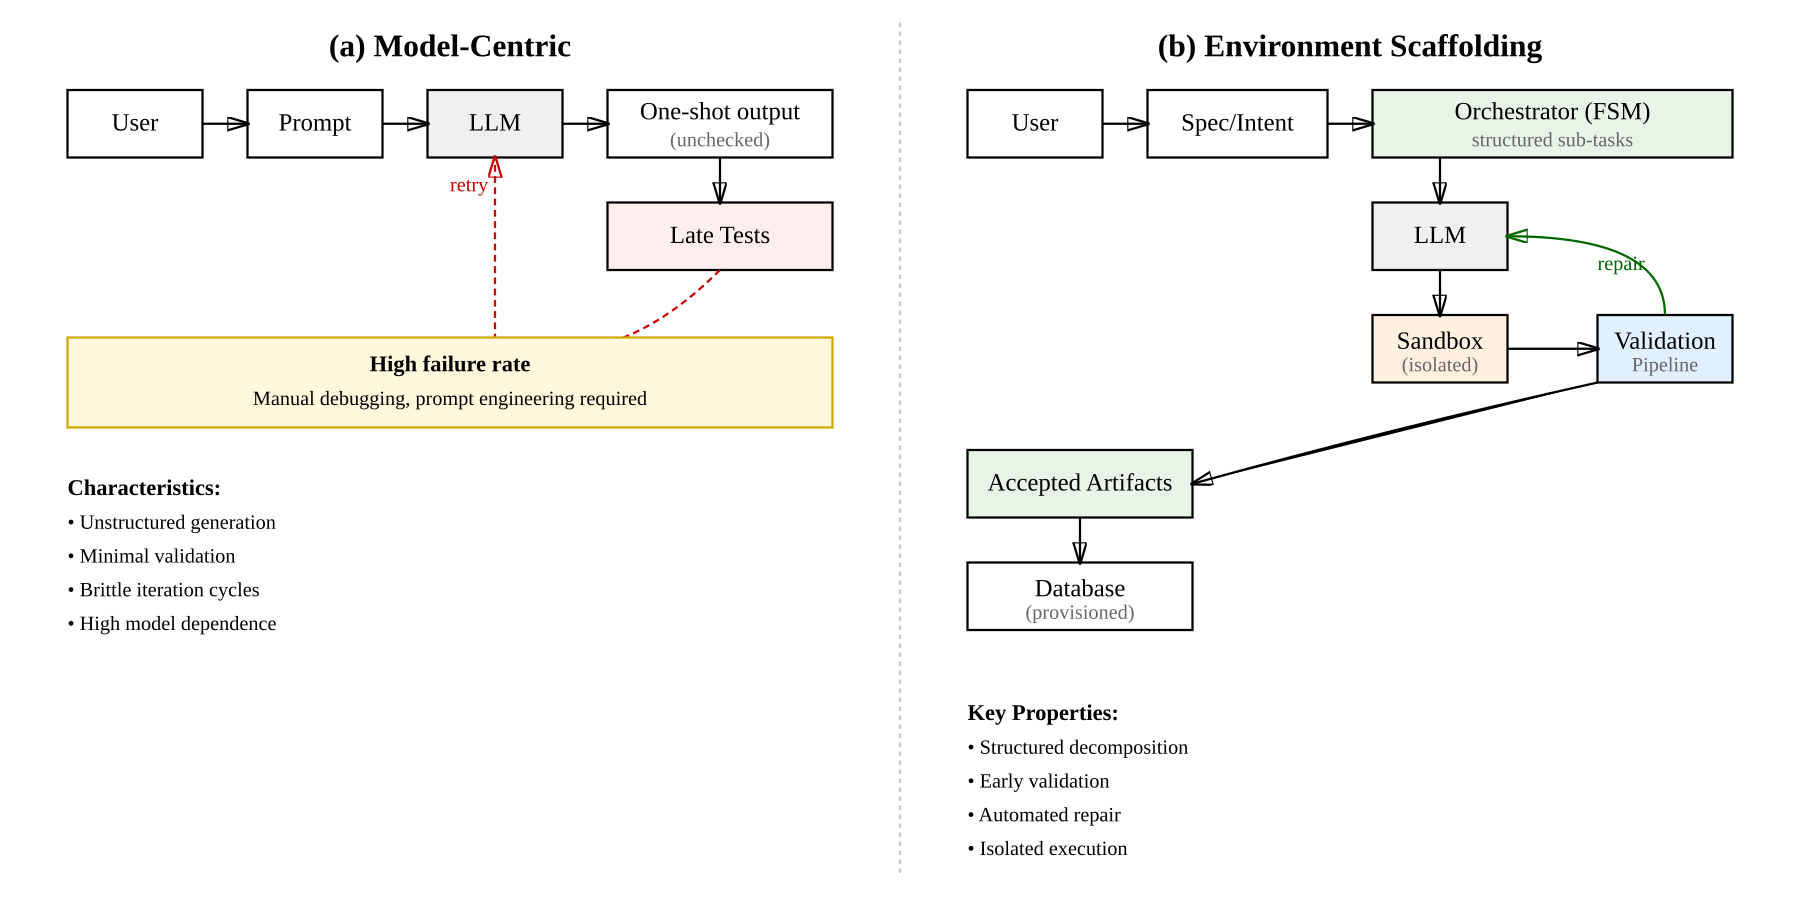
\includegraphics[width=\linewidth]{diagrams/es-vs-model.png}
  \vspace{-0.5em}
  \caption{\textbf{Environment scaffolding vs.\ model-centric generation.} ES wraps the model with a finite, validated workflow that catches errors early and repairs them before proceeding.}
  \label{fig:es-vs-model}
\end{figure}

\begin{table}[t]
\centering
\small
\begin{threeparttable}
\caption{\textbf{Environment scaffolding (ES) vs.\ model-centric generation.}}
\label{tab:es-contrast}
\begin{tabular}{@{}p{3.2cm}p{5.6cm}p{5.6cm}@{}}
\toprule
\textbf{Aspect} & \textbf{Model-Centric} & \textbf{Environment Scaffolding (Ours)} \\
\midrule
Task decomposition & Single/loosely guided multi-step; no fixed structure &
Explicit pipeline (FSM): schema $\rightarrow$ API $\rightarrow$ UI \\
Validation & Late or ad-hoc checks &
Integrated per-step: linters, type checks, unit/smoke tests \\
Error recovery & Manual/ad-hoc retries &
Automatic repair loop using error feedback \\
Execution isolation & Often none; runs on host &
Isolated containers; reproducible runs \\
Model dependence & Strong (prompt/model specific) &
Model-agnostic; environment guides behavior \\
Observability & Limited, coarse logs &
Per-step metrics, artifacts, and logs \\
\bottomrule
\end{tabular}
\end{threeparttable}
\end{table}

\subsection{Contributions}

Our work advances \emph{environment-first} agent design. The main contributions are:

\begin{itemize}
  \item \textbf{Environment Scaffolding Paradigm.} We formalize \emph{environment scaffolding (ES)} and show how structuring the action space with per-step validation enables reliable code generation without model-specific tricks.
  \item \textbf{Open-Source Framework (app.build).} We release an implementation of ES that targets three stacks (TypeScript/tRPC, PHP/Laravel, Python/NiceGUI) and ships with validators and deployment hooks.\footnote{See repository overview for supported stacks and validators.}
  \item \textbf{Empirical Evaluation.} Across end-to-end app-building tasks, we quantify the effect of validation layers and iterative repair, and compare multiple LLM backends under the same environment.
  \item \textbf{Methodological Insight.} We find that improving the \emph{environment} (constraints, tests, repair loops) often matters more than scaling the model for production reliability.
  \item \textbf{Community Adoption.} The framework has been used to generate thousands of applications in practice, suggesting ES is useful beyond controlled experiments.
\end{itemize}

\section{Background and Related Work}
\label{sec:related}

\subsection{Agentic Software Engineering}

The evolution of AI coding agents has progressed from simple code completion to autonomous software engineering systems capable of repository-level modifications. \textbf{SWE-bench} \citep{jimenez2024swe} established the gold standard for evaluating repository-level understanding with 2,294 real GitHub issues from 12 Python projects. The accompanying \textbf{SWE-agent} \citep{yang2024swe} demonstrated that custom agent-computer interfaces significantly enhance performance, achieving 12.5\% pass@1 through careful interface design rather than model improvements.

Repository-level agents have emerged as a distinct research direction. \textbf{WebArena} \citep{zhou2024webarena} revealed that even GPT-4 achieves only 14.41\% success versus 78.24\% human performance in realistic environments, demonstrating that environment design matters more than model capability. \textbf{GAIA} \citep{mialon2023gaia} reinforces this with 92\% human versus 15\% GPT-4 performance on practical tasks. \textbf{AutoCodeRover} \citep{zhang2024autocoder} combines LLMs with spectrum-based fault localization, achieving 19\% efficacy on SWE-bench at \$0.43 per issue. More recently, \textbf{Agentless} \citep{xia2024agentless} challenged complex agent architectures with a simple three-phase process (localization, repair, validation) achieving 32\% on SWE-bench Lite at \$0.70 cost, suggesting that sophisticated architectures may not always improve performance.

\textbf{Multi-agent systems} have consistently outperformed single-agent approaches. \textbf{AgentCoder} \citep{huang2023agentcoder} employs a three-agent architecture (Programmer, Test Designer, Test Executor) achieving 96.3\% pass@1 on HumanEval with GPT-4, compared to 71.3\% for single-agent approaches. \textbf{MapCoder} \citep{islam2024mapcoder} extends this with four specialized agents replicating human programming cycles, achieving 93.9\% pass@1 on HumanEval and 22.0\% on the challenging APPS benchmark. \textbf{MetaGPT} \citep{hong2023metagpt} demonstrates role-based agents communicating through structured documents, achieving 85.9\% pass@1 on HumanEval with 100\% task completion on software development tasks.

\subsection{Production Quality in Generated Code}

Ensuring production-ready AI-generated code requires validation approaches beyond simple correctness testing. \textbf{Static analysis integration} has shown promise, with intelligent code analysis agents combining GPT-3/4 with traditional static analysis to reduce false-positive rates from 85\% to 66\%. \textbf{Testing frameworks} have evolved to address AI-specific challenges. Test-driven approaches like TiCoder achieve 45.97\% absolute improvement in pass@1 accuracy through interactive generation. Property-based testing frameworks show 23.1--37.3\% relative improvements over established TDD methods by generating tests that capture semantic properties rather than specific implementations.

\textbf{AST-based validation} provides structural correctness guarantees. AST-T5 leverages Abstract Syntax Trees for structure-aware analysis, outperforming CodeT5 by 2--3 points on various tasks. Industry deployment reveals gaps between offline performance and practical usage. CodeAssist collected 2M completions from 1,200+ users over one year, revealing significant discrepancies between benchmark performance and real-world usage patterns.

\subsection{Tree Search}

Tree search enhances LLM-based solutions and serves as a way to increase compute budget beyond internal model reasoning token budget. The closest approach is used by Li et al. in S* Scaling \citep{li2025s} by combining iterative feedback with parallel branches taking different paths toward solving the problem. Sampling more trajectories increases success rate significantly, which is evident by difference in pass@1 and pass@3 often by 30\% or more.

\subsection{Runtime Isolation and Scaling}
Sandboxing is a cornerstone due to web applications requiring much more elaborate testing than running unit tests. It includes setup and teardown of databases and browser emulation. To run that in parallel for scaling we opted for Dagger.io for its caching capabilities and compatibility with Docker.

\section{Problem Setup and Method}
\label{sec:method}

\subsection{Problem Formulation}

LLM-based code generation enables rapid prototyping but often produces code that does not meet production standards. We formalize this as an environment design problem where success depends not just on model capability but on the structured constraints and validation feedback provided by the generation environment.

\subsection{Architecture}

\textbf{High-level design.} The app.build agent implements ES with a central \emph{orchestrator} that decomposes a user's specification into stack-specific stages and executes each stage inside an isolated sandbox with validation before acceptance. The same workflow applies across supported stacks (TypeScript/tRPC, PHP/Laravel, Python/NiceGUI). Per-stage validators are stack-aware (e.g., ESLint+TypeScript and Playwright for tRPC; PHPStan and feature/architecture tests for Laravel; \texttt{pytest}/\texttt{ruff}/\texttt{pyright} for Python data apps), and the platform provisions a managed Postgres database and CI/CD hooks for each generated project.

\begin{figure}[t]
  \centering
  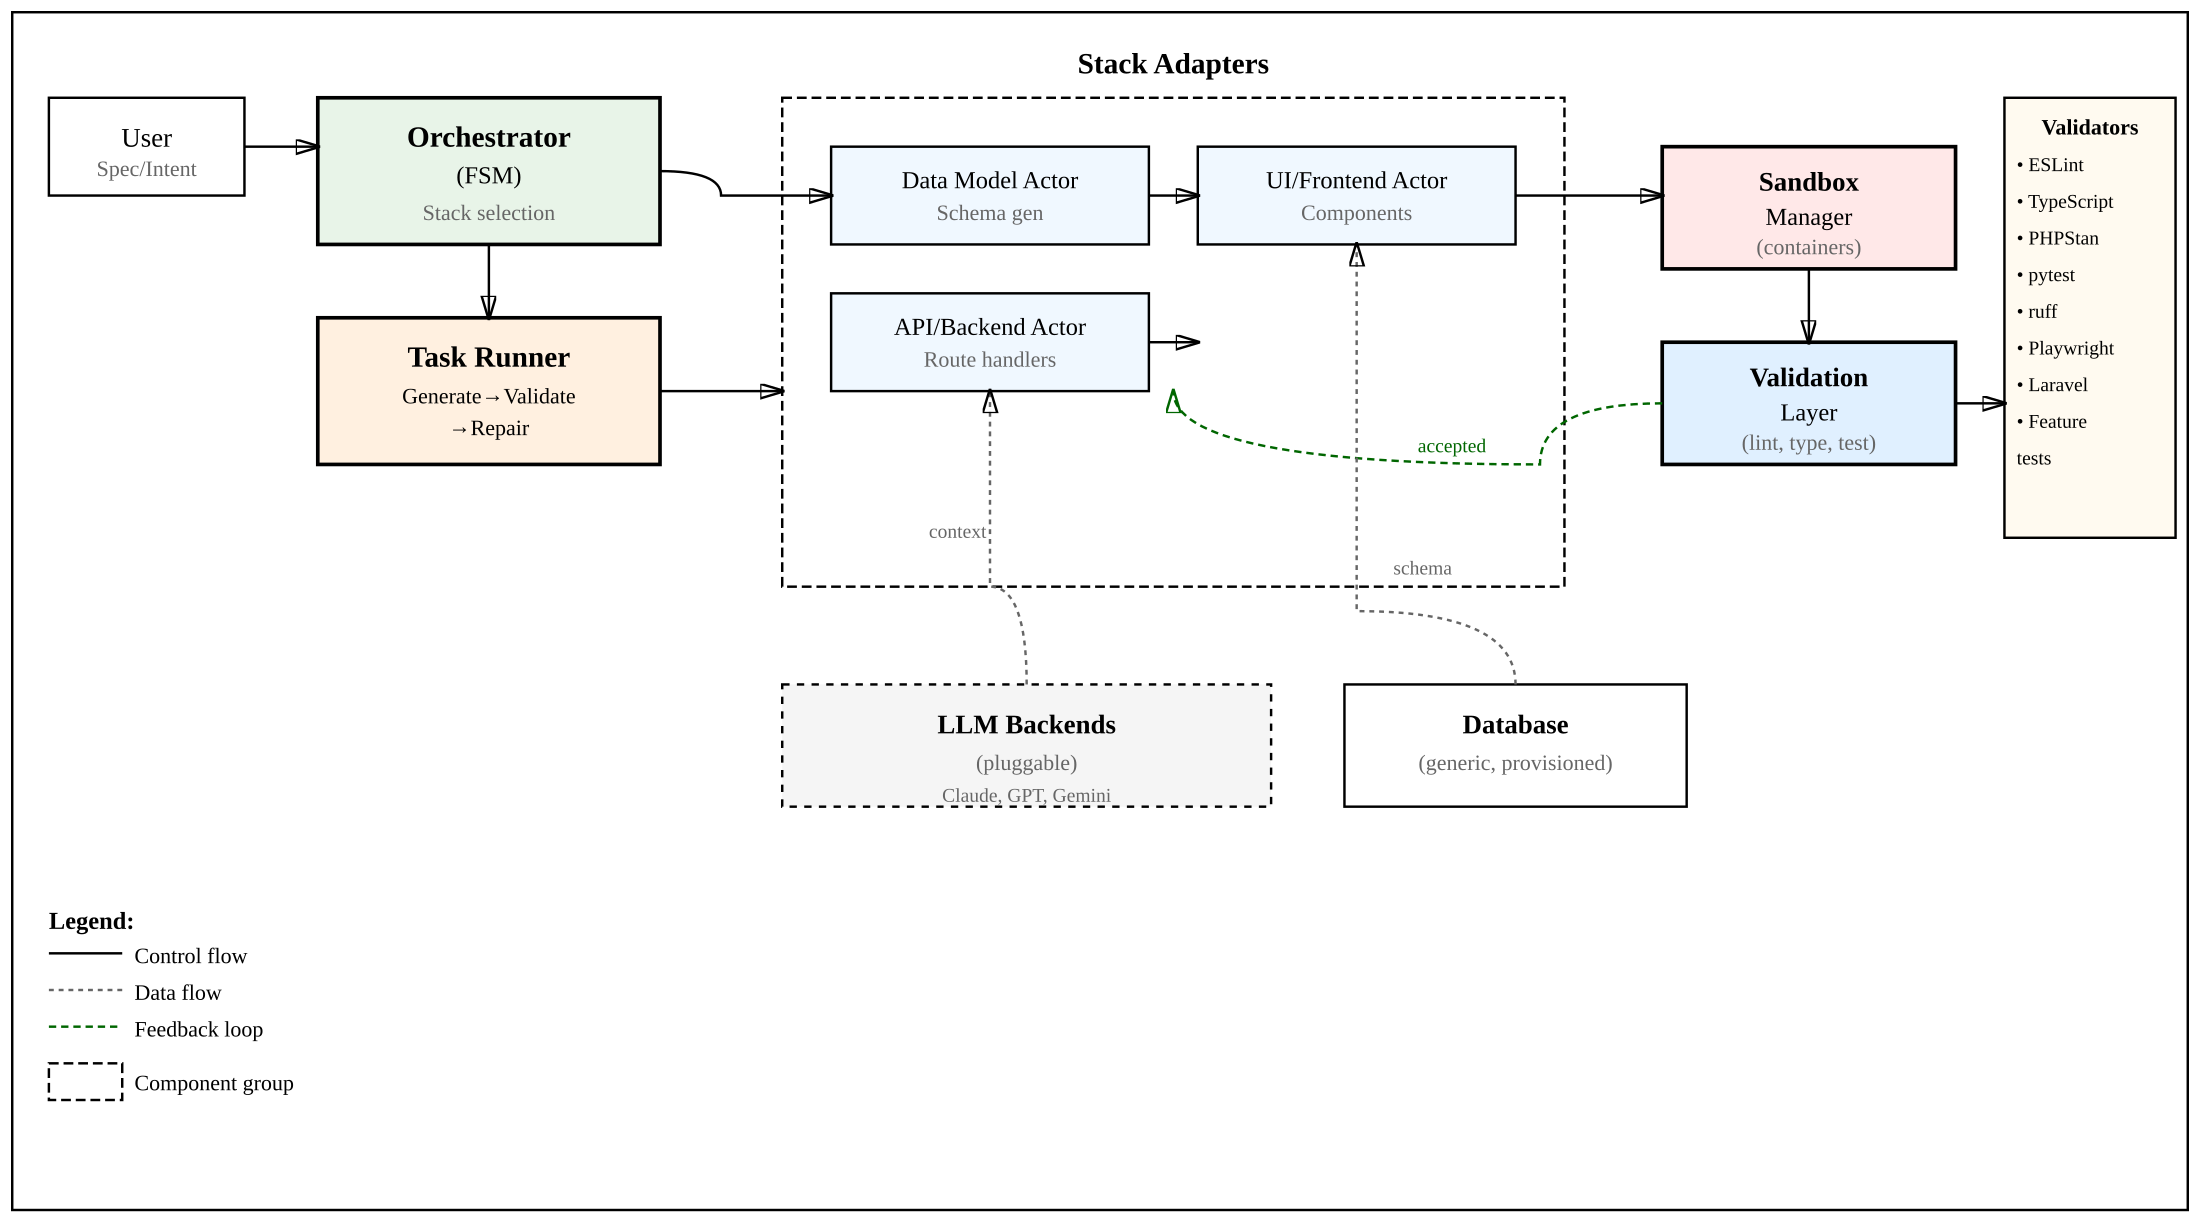
\includegraphics[width=\linewidth]{diagrams/appbuild-arch.png}
  \vspace{-0.5em}
  \caption{\textbf{app.build architecture} expressed through environment scaffolding. The orchestrator plans stages per stack; each sub-task runs in a sandbox, is validated, and only then merged. CI/CD and DB provisioning are integrated.}
  \label{fig:appbuild-arch}
\end{figure}

\textbf{Execution loop.} For each sub-task, the agent (i) assembles minimal context (files, interfaces, constraints), (ii) prompts the LLM, (iii) executes the result in a sandbox, (iv) collects validator feedback, and (v) either accepts the artifact or re-prompts to repair. This iterative loop provides robustness without assuming a particular model, and scales by parallelizing sandboxes and caching environment layers.

\section{Experimental Setup}
\label{sec:experimental-setup}

In order to support claims in this paper and validate specific design decisions for supported stacks, we designed a set of experiments based on a specially created prompt dataset and metrics designed to evaluate viability and quality of generated applications.

\subsection{Evaluation Framework}

\subsection{Prompt Dataset}
\label{sec:prompt-dataset-desc}

The evaluation dataset comprises 30 prompts designed to assess system performance across diverse application development scenarios. Evaluation prompts were created involving independent human contributors with no prior exposure to the app.build system architecture. Contributors developed tasks reflecting authentic development workflows from their professional experience. The prompts were subsequently filtered to exclude items requiring enterprise integrations, significant compute resources for AI/ML, or other capabilities beyond the framework's scope. Raw prompts underwent automated post-processing using LLMs to anonymize sensitive information and standardize linguistic structure.
The resulting dataset consists of 30 prompts spanning a complexity spectrum (low: static/single-page UI; medium: single-entity CRUD; high: multi-entity/custom logic).
See the full list of prompts in Appendix~\ref{sec:prompt-dataset}.

\subsection{Metrics}

Each application generated by the agent was evaluated by the following metrics, designed to assess its viability and quality under preset time and cost constraints.

\begin{itemize}
\item Viability rate ($V=1$) and non-viability rate ($V=0$)
\item Perfect quality rate ($Q=10$) and quality distribution (mean/median for $V=1$ apps)
\item Validation pass rates by check (AB-01, AB-02, AB-03, AB-04, AB-06, AB-07)
\item Quality scores ($Q$, 0--10) using the rubric in Section~\ref{sec:scoring}
\item Model/cost comparisons where applicable
\end{itemize}

\subsection{Experimental Configurations}

We designed three experimental configurations to systematically evaluate factors affecting app generation success rates:

\textbf{Configuration 1: Baseline}. We generated baseline tRPC apps with default production setup and all checks ON to assess default generation success rate, cost and time.

\textbf{Configuration 2: Model Architecture Analysis}. Using the tRPC stack, we evaluated open versus closed foundation models. Claude Sonnet 4 served as the baseline coding model, compared against Qwen3-Coder-480B-A35B \citep{qwen2025qwen3} and GPT OSS 120B \citep{openai2025gpt} as open alternatives.

\textbf{Configuration 3: Testing Framework Ablation}. We conducted three ablation studies on the tRPC stack isolating the impact of each type of checks by turning them off independently: (3a) disabled isolated Playwright UI smoke tests; (3b) disabled ESLint checks; and (3c) removed handlers tests, eliminating backend validation.

\subsection{Assessor Protocol and Scoring}
\label{sec:scoring}

To systematically assess generated application quality, we implement a structured evaluation protocol comprising six standardized functional checks executed by human assessors. The evaluation reports two independent outcomes: a binary viability indicator ($V$) and a 0--10 quality score ($Q$).

\textbf{Viability (binary)}:
\begin{equation}
V = \begin{cases}
1 & \text{if AB-01 and AB-02 are not FAIL} \\
0 & \text{otherwise}
\end{cases}
\end{equation}

\textbf{Quality (0--10)}:
\begin{equation}
Q = 10 \times \frac{\sum_{c \in A} w \times s_c}{\sum_{c \in A} w}
\end{equation}

where $A$ is the set of applicable checks (excluding NA); all checks use equal weights prior to NA re-normalization; and per-check grades $s_c$ are mapped as follows:
\begin{itemize}
\item AB-01 (Boot): PASS = 1.0, WARN = 0.5, FAIL = 0.0
\item AB-02 (Prompt correspondence): PASS = 1.0, WARN = 0.5, FAIL = 0.0
\item AB-03, AB-04, AB-06 (Clickable Sweep): PASS = 1.0, WARN = 0.5, FAIL = 0.0
\item AB-07 (Performance): continuous metric normalized to $[0,1]$
\end{itemize}

\begin{table}[t]
\caption{Check weights and definitions used in scoring (see rubric in Section~\ref{sec:scoring}). All checks share equal weight after NA re-normalization; AB-01 and AB-02 are hard gates for Viability $V$.}
\label{tab:check-weights}
\centering
\begin{threeparttable}
\begin{tabular}{llcl}
\toprule
Check ID & Check Description & Weight (share) & Notes \\
\midrule
AB-01 & Boot \& Home & 1/6 & Hard gate for Viability $V$ \\
AB-02 & Prompt Correspondence & 1/6 & Hard gate for Viability $V$ \\
AB-03 & Create Functionality & 1/6 &  \\
AB-04 & View/Edit Operations & 1/6 &  \\
AB-06 & Clickable Sweep & 1/6 &  \\
AB-07 & Performance Metrics & 1/6 & Continuous; normalized to $[0,1]$ \\
\bottomrule
\end{tabular}
\begin{tablenotes}
\item \textit{Note.} See mapping of PASS/WARN/FAIL to numeric scores and viability definition in Section~\ref{sec:scoring}.
\end{tablenotes}
\end{threeparttable}
\end{table}

\section{Results}
\label{sec:results}

\subsection{Environment Scaffolding Impact (TypeScript/tRPC only)}

Evaluating 30 TypeScript/tRPC applications, we observe that 70.0\% (21/30) achieved viability ($V=1$), with 30.0\% attaining perfect quality ($Q=10$) and 30.0\% non-viable ($V=0$). Once viability criteria are met, generated applications exhibit consistently high quality.

\begin{table}[t]
\caption{Aggregated evaluation results for TypeScript/tRPC ($n=30$ prompts). Viability $V$ and quality $Q$ are defined in Section~\ref{sec:scoring}. ``Perfect quality'' denotes $Q=10$ (all applicable checks PASS). ``Non-viable'' denotes $V=0$ (AB-01 or AB-02 = FAIL). Mean quality is computed over viable apps only ($V=1$).}
\label{tab:aggregated-results}
\centering
\begin{threeparttable}
\begin{tabular}{llc}
\toprule
Metric & Value & Key Insight \\
\midrule
Total Applications & 30 & TypeScript/tRPC stack only \\
Viability Rate ($V=1$) & 70.0\% & 21/30 viable applications \\
Perfect Quality ($Q=10$) & 30.0\% & 9/30 fully compliant applications \\
Non-viable ($V=0$) & 30.0\% & 9/30 failed smoke tests \\
Mean Quality ($V=1$ apps) & 8.78 & High quality when viable \\
\bottomrule
\end{tabular}
\begin{tablenotes}
\item \textit{Note.} Scoring rubric and check definitions in Section~\ref{sec:scoring}.
\end{tablenotes}
\end{threeparttable}
\end{table}

\begin{table}[t]
\caption{Check-specific outcomes across $n=30$ TypeScript/tRPC tasks. See Section~\ref{sec:scoring} for check definitions, PASS/WARN/FAIL grading, and the viability rule. NA indicates the check was not applicable to a prompt (e.g., AB-04 when no view/edit flows are required). ``Pass Rate (excl. NA)'' is computed over applicable cases only.}
\label{tab:check-pass-rates}
\centering
\begin{threeparttable}
\begin{tabular}{lccccc}
\toprule
Check & Pass & Warn & Fail & NA & Pass Rate (excl. NA) \\
\midrule
AB-01 (Boot) & 25 & 2 & 3 & 0 & 83.3\% \\
AB-02 (Prompt) & 19 & 3 & 5 & 3 & 70.4\% \\
AB-03 (Create) & 22 & 2 & 0 & 6 & 91.7\% \\
AB-04 (View/Edit) & 17 & 1 & 1 & 11 & 89.5\% \\
AB-06 (Clickable Sweep) & 20 & 4 & 1 & 5 & 80.0\% \\
AB-07 (Performance) & 23 & 3 & 0 & 4 & 88.5\% \\
\bottomrule
\end{tabular}
\begin{tablenotes}
\item \textit{Note.} AB-07 is a continuous metric normalized to $[0,1]$; thresholding for PASS/WARN/FAIL is specified in Section~\ref{sec:scoring}.
\end{tablenotes}
\end{threeparttable}
\end{table}

Smoke tests (AB-01, AB-02) determine viability. Among viable applications ($V=1$, $n=21$), quality averaged 8.78 with 77.3\% achieving $Q \geq 9$. Non-viability ($V=0$) arises from smoke test failures or missing artifacts.

\subsection{Open vs Closed Model Performance}

We evaluated Claude Sonnet 4 against two open-weights models using the TypeScript/tRPC stack with full validation pipelines. Claude achieved 86.7\% success rate, establishing our closed-model baseline at \$110.20 total cost. Qwen3-Coder-480B-A35B reached 70\% success rate (80.8\% relative performance) while GPT OSS 120B managed only 30\% success rate. Both open models were accessed via OpenRouter, resulting in significantly lower costs: \$12.68 for Qwen3 and \$4.55 for GPT OSS.

The performance gap reveals that environment scaffolding alone cannot eliminate the need for capable foundation models. However, leading open-weights models like Qwen3 demonstrate that structured environments can enable production-viable performance at substantially reduced costs. The 9x cost reduction for 19\% performance loss represents a viable tradeoff for cost-sensitive deployments.

Operational characteristics differed notably between model types. Open models required more validation retries, evidenced by higher LLM call counts (4,359 for Qwen3, 4,922 for GPT OSS vs 3,413 for Claude). Healthcheck pass rates (86.7\% for Qwen3 vs 96.7\% for Claude) indicate that open models generate syntactically correct code but struggle more with integration-level correctness, emphasizing the importance of comprehensive validation pipelines for open-weights deployments.

\subsection{Ablation Studies: Impact of Validation Layers}

To understand how each validation layer contributes to application quality, we conducted controlled ablations on the same 30-prompt cohort. Each ablation removes one validation component while keeping others intact.

\textbf{Baseline Performance} (all validation layers active):
\begin{itemize}
\item Viability: 73.3\% (22/30 apps pass both AB-01 Boot and AB-02 Prompt)
\item Mean Quality: 8.06 (among all 30 apps)
\end{itemize}

\textbf{Finding 1: Removing Unit Tests Trades Quality for Viability}
\begin{itemize}
\item Viability: 80.0\% (+6.7 pp) -- fewer apps fail smoke tests
\item Mean Quality: 7.78 ($-0.28$) -- quality degrades despite higher viability
\item Key degradations: AB-04 View/Edit drops from 90\% to 60\% pass rate ($-30$ pp)
\item Interpretation: Backend tests catch critical CRUD errors. Without them, apps boot successfully but fail on data operations.
\end{itemize}

\textbf{Finding 2: Removing Linting Has Mixed Effects}
\begin{itemize}
\item Viability: 80.0\% (+6.7 pp)
\item Mean Quality: 8.25 (+0.19) -- slight improvement
\item Trade-offs: AB-03 Create drops 8.3 pp, AB-04 View/Edit drops 7.6 pp
\item Interpretation: ESLint catches legitimate issues but may also block valid patterns. The performance gain suggests some lint rules may be overly restrictive.
\end{itemize}

\textbf{Finding 3: Removing Playwright Tests Significantly Improves Outcomes}
\begin{itemize}
\item Viability: 90.0\% (+16.7 pp) -- highest among all configurations
\item Mean Quality: 8.62 (+0.56) -- meaningful quality improvement
\item Broad improvements: AB-02 Prompt +11.8 pp, AB-06 Clickable +5.7 pp
\item Interpretation: Playwright tests appear overly brittle for scaffolded apps. Many apps that fail E2E tests actually work correctly for users. The 36 improved vs 6 regressed cases for AB-02 support this interpretation.
\end{itemize}

\subsection{Synthesis: Optimal Validation Strategy}

Our ablation results reveal clear trade-offs in validation design:

\textbf{Validation Layer Impact Summary}:
\begin{enumerate}
\item \textbf{Unit/Handler Tests}: Essential for data integrity. Removing them increases perceived viability but causes real functional regressions (especially AB-04 View/Edit).
\item \textbf{ESLint}: Provides modest value with some false positives. The small quality impact (+0.19) and mixed per-dimension effects suggest selective application.
\item \textbf{Playwright/E2E}: Currently causes more harm than good. The +16.7 pp viability gain and quality improvements indicate these tests reject too many working applications.
\end{enumerate}

\textbf{Recommended Validation Architecture}:
Based on these findings, we recommend:
\begin{itemize}
\item \textbf{Keep}: Lightweight smoke tests (boot + primary route), backend unit tests for CRUD operations
\item \textbf{Refine}: ESLint with curated rules focusing on actual errors vs style preferences
\item \textbf{Replace}: Full E2E suite with targeted integration tests for critical paths only
\end{itemize}

This pragmatic approach balances catching real defects while avoiding false rejections of functional applications. Importantly, when quality is paramount and compute budget less constrained (our experimental budget was capped), comprehensive validation including strict E2E tests remains a viable strategy--trading lower success rates for guaranteed production quality.

\subsection{Failure Mode Analysis}

Observed failure modes in tRPC runs cluster into categories:

\begin{itemize}
\item \textbf{Boot/Load failures}: template placeholders or incomplete artifacts
\item \textbf{Prompt correspondence failures}: generic template likely because of generation failure
\item \textbf{CSP/security policy restrictions}: blocked images or media by default policies
\item \textbf{UI interaction defects}: unbound handlers, non-working controls
\item \textbf{State/integration defects}: data not persisting across refresh; broken filters; login issues
\item \textbf{Component misuse}: runtime exception due to incorrect component composition
\end{itemize}

These defects align with our layered pipeline design: early gates catch non-viable builds, while later gates expose interaction/state issues before human evaluation.

\subsection{Prompt Complexity and Success Rate}
\label{sec:prompt-complexity}

We categorize prompts along a simple rubric and analyze success impacts:

\begin{itemize}
\item \textbf{Low complexity}: static or single-page UI tasks (e.g., landing pages, counters)
\item \textbf{Medium complexity}: single-entity CRUD without advanced flows or auth
\item \textbf{High complexity}: multi-entity workflows, custom logic, or complex UI interactions
\end{itemize}

Empirically, medium-complexity CRUD prompts achieve the highest quality ($Q=9$--10 typical), reflecting strong scaffolding for data models and handlers. Low-complexity UI prompts are not uniformly ``easy'': several became non-viable ($V=0$) by failing prompt correspondence (AB-02) with generic templates. High-complexity prompts show lower viability rates due to interaction wiring and state-consistency issues surfaced by AB-04/AB-06.

\section{Discussion}
\label{sec:discussion}

\subsection{Limitations}
\label{sec:limitations}

Our current framework is limited to CRUD-oriented data applications, focusing on structured workflows with well-defined input-output expectations. While effective for common web application patterns, it does not yet support complex systems or advanced integrations. The validation pipeline, though comprehensive, relies on domain-specific heuristics and expert-defined anti-patterns, which may not generalize to novel or edge-case designs. Additionally, our human evaluation protocol, while rigorous, is poorly scalable and constrained by subjectivity in assessing maintainability and user experience nuances.

\subsection{Broader Impact}
\label{sec:broader-impact}

The AI agent boom is accelerating, but real industry deployments often fail silently. Without environment scaffolding, we risk massive overengineering of AI models while ignoring the real bottleneck. App.build represents a shift from model-centric to system-centric AI engineering--a critical step toward scaling reliable agent environments. As emphasized in Machine Learning System Design with End-to-End Examples \citep{babushkin2025machine}, production AI systems only become effective when development integrates not just model performance, but core software engineering principles. By open-sourcing both the framework and evaluation protocol, we provide a reproducible, transparent foundation for building and benchmarking agent environments at scale.

\section{Conclusion}
\label{sec:conclusion}

Our results demonstrate that raw model capability alone cannot bridge the gap between AI potential and production reality. Through systematic environment scaffolding, multi-layered validation, and stack-specific orchestration, app.build transforms probabilistic language models into dependable software engineering agents.

Ablations indicate clear trade-offs across validation layers: removing unit/handlers tests increases apparent viability but reduces CRUD/view-edit correctness; removing linting yields small viability/performance gains with modest quality regressions; removing Playwright smoke improves viability and observed quality, likely by eliminating flaky UI checks for scaffolded apps. Together, these results support a pragmatic stance: retain minimal, targeted smoke to guarantee boot and primary flows; keep structural checks (lint) to preserve UI/code consistency; and scope E2E to a ``golden path'' to avoid false negatives while still catching session/flow breakage.

We conclude that the path to reliable, production-ready AI agents lies not in better prompts or bigger models, but in principled, scalable environment engineering, with validation layers tuned to maximize developer-visible value while minimizing brittleness.

\section*{Acknowledgments}

This submission is prepared in collaboration between app.build (Databricks - app.build team) and THWS University of Applied Sciences W\"urzburg-Schweinfurt (CAIRO). We thank the app.build community for their contributions and feedback. Special thanks to Databricks executive team for supporting the open-source initiative.

\section*{References}

% Note: For actual submission, you would use natbib for references
% Here we include references inline for demonstration

\small

[1] Austin, J., et al. (2021). Program synthesis with large language models. \textit{arXiv preprint arXiv:2108.07732}.

[2] Babushkin, V. \& Kravchenko, A. (2025). Machine Learning System Design with End-to-End Examples. Manning Publications.

[3] Chen, M., et al. (2021). Evaluating Large Language Models Trained on Code. \textit{arXiv preprint arXiv:2107.03374}.

[4] Cognition Labs. (2024). SWE-bench Technical Report. \url{https://cognition.ai/blog/swe-bench-technical-report}

[5] Hong, S., et al. (2023). MetaGPT: Meta Programming for A Multi-Agent Collaborative Framework. \textit{arXiv preprint arXiv:2308.00352}.

[6] Huang, D., et al. (2023). AgentCoder: Multi-Agent-based Code Generation with Iterative Testing and Optimisation. \textit{arXiv preprint arXiv:2312.13010}.

[7] Islam, M. A., et al. (2024). MapCoder: Multi-Agent Code Generation for Competitive Problem Solving. \textit{arXiv preprint arXiv:2405.11403}.

[8] Jiang, J., et al. (2024). A Survey on Large Language Models for Code Generation. \textit{arXiv preprint arXiv:2406.00515}.

[9] Jimenez, C., et al. (2024). SWE-bench: Can Language Models Resolve Real-World GitHub Issues? \textit{arXiv preprint arXiv:2310.06770}.

[10] Li, et al. (2025). S*: Test Time Scaling for Code Generation. \textit{arXiv preprint arXiv:2502.14382}.

[11] Liu, J., et al. (2023). Is Your Code Generated by ChatGPT Really Correct? Rigorous Evaluation of Large Language Models for Code Generation. \textit{arXiv preprint arXiv:2305.01210}.

[12] Mialon, G., et al. (2023). GAIA: A Benchmark for General AI Assistants. \textit{ICLR}.

[13] OpenAI. (2025). gpt-oss-120b \& gpt-oss-20b Model Card. \textit{arXiv preprint arXiv:2508.10925}.

[14] Paul, D. et al. (2024). Benchmarks and Metrics for Evaluations of Code Generation: A Critical Review. \textit{arXiv preprint arXiv:2406.12655}.

[15] Qwen Team. (2025) Qwen3 Technical Report. \textit{arXiv preprint arXiv:2505.09388}.

[16] Xia, C. S., et al. (2024). Agentless: Demystifying LLM-based Software Engineering Agents. \textit{arXiv preprint arXiv:2407.01489}.

[17] Yang, J., et al. (2024). SWE-agent: Agent-Computer Interfaces Enable Automated Software Engineering. \textit{arXiv preprint arXiv:2405.15793}.

[18] Zhang, R., et al. (2023). R-Tuning: Instructing Large Language Models to Say 'I Don't Know'. \textit{arXiv preprint arXiv:2311.09677}.

[19] Zhang, Y., et al. (2024). AutoCodeRover: Autonomous Program Improvement. \textit{arXiv preprint arXiv:2404.05427}.

[20] Zhou, S., et al. (2024). WebArena: A Realistic Web Environment for Building Autonomous Agents. \textit{ICLR}.

%%%%%%%%%%%%%%%%%%%%%%%%%%%%%%%%%%%%%%%%%%%%%%%%%%%%%%%%%%%%

\appendix

\section{Prompt Dataset (Full List)}
\label{sec:prompt-dataset}

\begin{table}[h]
\caption{Complete prompt dataset used in evaluation ($n=30$). Dataset construction details in Section~\ref{sec:prompt-dataset-desc}. Complexity labels follow the rubric in Section~\ref{sec:prompt-complexity}: \emph{Low} (static/single-page UI), \emph{Medium} (single-entity CRUD), \emph{High} (multi-entity/custom logic).}
\label{tab:prompt-dataset}
\centering
\scriptsize
\begin{tabular}{p{3cm}p{8cm}p{1.5cm}}
\toprule
ID & Prompt (summary) & Complexity \\
\midrule
plant-care-tracker & Track plant conditions using moods with custom rule-based logic. No AI/ML/APIs. & Medium \\
roommate-chore-wheel & Randomly assigns chores weekly and tracks completion. & Medium \\
car-maintenance-dashboard & Monitor car maintenance history and upcoming service dates. & Medium \\
city-trip-advisor & Suggest tomorrow's trip viability based on weather forecast API. & High \\
currency-converter & Convert currency amounts using Frankfurter API. & Low \\
book-library-manager & Manage book library with CRUD operations, search, and filters. & Medium \\
wellness-score-tracker & Input health metrics, get daily wellness score with trends. & High \\
event-tracker & Basic event tracker with add, view, delete functionality. & Low \\
daily-pattern-visualizer & Log and visualize daily patterns (sleep, work, social time). & High \\
pantry-inventory-app & Track pantry items, expiry notifications, AI recipe suggestions. & High \\
home-lab-inventory & Catalog home lab infrastructure (hardware, VMs, IP allocations). & High \\
basic-inventory-system & Small business inventory with stock in/out transactions. & Medium \\
pastel-blue-notes-app & Notes app with pastel theme, folders, user accounts. & Medium \\
teacher-question-bank & Question bank with quiz generation and export features. & High \\
beer-counter-app & Single-page beer counter with local storage. & Low \\
plumbing-business-landing-page & Professional landing page for lead generation. & Low \\
kanji-flashcards & Kanji learning with SRS, progress tracking, JLPT levels. & High \\
bookmark-management-app & Save, tag, organize links with search and sync. & Medium \\
personal-expense-tracker & Log expenses, categories, budgets, spending visualization. & Medium \\
gym-crm & Gym CRM for class reservations with admin interface. & High \\
todo-list-with-mood & To-do list combined with mood tracker. & Medium \\
birthday-wish-app & Static birthday card with message and animation. & Low \\
pc-gaming-niche-site & Budget gaming peripherals review site with CMS. & Medium \\
tennis-enthusiast-platform & Social platform for finding tennis partners. & High \\
engineering-job-board & Niche job board for engineering positions. & High \\
indonesian-inventory-app & Inventory management app in Indonesian language. & Medium \\
habit-tracker-app & Track habits, daily progress, visualize streaks. & Medium \\
recipe-sharing-platform & Community platform for sharing recipes. & High \\
pomodoro-study-timer & Minimalistic Pomodoro timer with session logging. & Low \\
cat-conspiracy-tracker & Humorous app tracking cat suspicious activities. & Low \\
\bottomrule
\end{tabular}
\end{table}

%%%%%%%%%%%%%%%%%%%%%%%%%%%%%%%%%%%%%%%%%%%%%%%%%%%%%%%%%%%%

\newpage
\section*{NeurIPS Paper Checklist}

The checklist is designed to encourage best practices for responsible machine learning research, addressing issues of reproducibility, transparency, research ethics, and societal impact. The checklist should follow the references and follow the (optional) supplemental material. The checklist does NOT count towards the page limit.

Please read the checklist guidelines carefully for information on how to answer these questions. For each question in the checklist:
\begin{itemize}
    \item You should answer \textbf{Yes}, \textbf{No}, or \textbf{N/A}.
    \item \textbf{N/A} means either that the question is Not Applicable for that particular paper or the relevant information is Not Available.
    \item Please provide a short (1--2 sentence) justification right after your answer (even for N/A).
\end{itemize}

The checklist answers are an integral part of your paper submission. They are visible to the reviewers, area chairs, senior area chairs, and ethics reviewers.

\begin{enumerate}

\item {\bf Claims}
    \item[] Question: Do the main claims made in the abstract and introduction accurately reflect the paper's contributions and scope?
    \item[] Answer: \textbf{Yes}
    \item[] Justification: The abstract and introduction clearly state our contributions regarding environment scaffolding for code generation agents, with specific claims supported by experimental results on 30 generation tasks.

\item {\bf Limitations}
    \item[] Question: Does the paper discuss the limitations of the work performed by the authors?
    \item[] Answer: \textbf{Yes}
    \item[] Justification: Section~\ref{sec:limitations} explicitly discusses limitations including restriction to CRUD applications, reliance on domain-specific heuristics, and scalability challenges of human evaluation.

\item {\bf Theory Assumptions and Proofs}
    \item[] Question: For each theoretical result, does the paper provide the full set of assumptions and a complete (and correct) proof?
    \item[] Answer: \textbf{N/A}
    \item[] Justification: This paper focuses on empirical evaluation of a practical system rather than theoretical contributions requiring formal proofs.

\item {\bf Experimental Result Reproducibility}
    \item[] Question: Does the paper fully disclose all the information needed to reproduce the main experimental results of the paper to the extent that it affects the main claims and/or conclusions of the paper (regardless of whether the code and data are provided or not)?
    \item[] Answer: \textbf{Yes}
    \item[] Justification: We provide detailed experimental configurations, evaluation protocols, and the complete prompt dataset. The framework is open-source with reference implementations.

\item {\bf Open access to data and code}
    \item[] Question: Does the paper provide open access to the data and code, with sufficient instructions to faithfully reproduce the main experimental results, as described in supplemental material?
    \item[] Answer: \textbf{Yes}
    \item[] Justification: The app.build framework is open-source, and we provide the complete evaluation dataset and protocols in Appendix~\ref{sec:prompt-dataset}.

\item {\bf Experimental Setting/Details}
    \item[] Question: Does the paper specify all the training and test details (e.g., data splits, hyperparameters, how they were chosen, type of optimizer, etc.) necessary to understand the results?
    \item[] Answer: \textbf{Yes}
    \item[] Justification: Section~\ref{sec:experimental-setup} provides comprehensive experimental setup including configurations, model choices, evaluation metrics, and detailed scoring protocols.

\item {\bf Experiment Statistical Significance}
    \item[] Question: Does the paper report error bars suitably and correctly defined or other appropriate information about the statistical significance of the experiments?
    \item[] Answer: \textbf{No}
    \item[] Justification: We report success rates and quality scores but do not include statistical significance tests due to the limited sample size (30 prompts) and focus on practical system evaluation rather than statistical inference.

\item {\bf Experiments Compute Resources}
    \item[] Question: For each experiment, does the paper provide sufficient information on the computer resources (type of compute workers, memory, time of execution) needed to reproduce the experiments?
    \item[] Answer: \textbf{Partial}
    \item[] Justification: We mention Dagger.io infrastructure and Docker-based sandboxing but do not provide detailed compute resource specifications for reproduction.

\item {\bf Code Of Ethics}
    \item[] Question: Does the research conducted in the paper conform, in every respect, with the NeurIPS Code of Ethics?
    \item[] Answer: \textbf{Yes}
    \item[] Justification: Our research focuses on improving software development tools and does not involve human subjects, sensitive data, or potential for misuse.

\item {\bf Broader Impacts}
    \item[] Question: Does the paper discuss both potential positive societal impacts and negative societal impacts of the work performed?
    \item[] Answer: \textbf{Yes}
    \item[] Justification: Section~\ref{sec:broader-impact} discusses the broader impact of shifting from model-centric to environment-centric AI engineering and the importance of production-ready agent systems.

\item {\bf Safeguards}
    \item[] Question: Does the paper describe safeguards that have been put in place for responsible release of data or models that have a high risk for misuse?
    \item[] Answer: \textbf{N/A}
    \item[] Justification: Our work involves a software development framework rather than models or datasets with high misuse potential.

\item {\bf Licenses for existing assets}
    \item[] Question: Are the creators or original owners of assets (e.g., code, data, models), used in the paper, properly credited and are the license and terms of use explicitly mentioned and properly respected?
    \item[] Answer: \textbf{Yes}
    \item[] Justification: We properly cite all referenced models, benchmarks, and tools. The app.build framework is released as open-source with appropriate licensing.

\item {\bf New Assets}
    \item[] Question: Are new assets introduced in the paper well documented and is the documentation provided alongside the assets?
    \item[] Answer: \textbf{Yes}
    \item[] Justification: The app.build framework and evaluation dataset are well-documented with detailed protocols provided in the appendix and open-source repository.

\item {\bf Crowdsourcing and Research with Human Subjects}
    \item[] Question: For crowdsourcing experiments and research with human subjects, does the paper include the full text of instructions given to participants and screenshots, if applicable, as well as details about compensation (if any)?
    \item[] Answer: \textbf{N/A}
    \item[] Justification: Our evaluation involved human assessors following standardized protocols but did not constitute formal human subjects research requiring IRB approval.

\item {\bf Institutional Review Board (IRB) Approvals or Equivalent for Research with Human Subjects}
    \item[] Question: Does the paper describe potential risks incurred by study participants, whether such risks were disclosed to the subjects, and whether Institutional Review Board (IRB) approvals were obtained?
    \item[] Answer: \textbf{N/A}
    \item[] Justification: The human evaluation did not involve study participants but rather standard software testing protocols by technical evaluators.

\end{enumerate}

\end{document}
